% Figure 1 of Paper D: the claim-registry verification loop.
% Built by scripts/generate_paper_d_figures.py (Tectonic -> PDF, pdftoppm -> PNG/TIFF).
\documentclass[border=6pt]{standalone}
\usepackage{fontspec}
\setmainfont{texgyretermes}[Extension=.otf, UprightFont=*-regular, BoldFont=*-bold,
  ItalicFont=*-italic, BoldItalicFont=*-bolditalic]
\usepackage{tikz}
\usetikzlibrary{positioning,arrows.meta,fit,calc}
\begin{document}
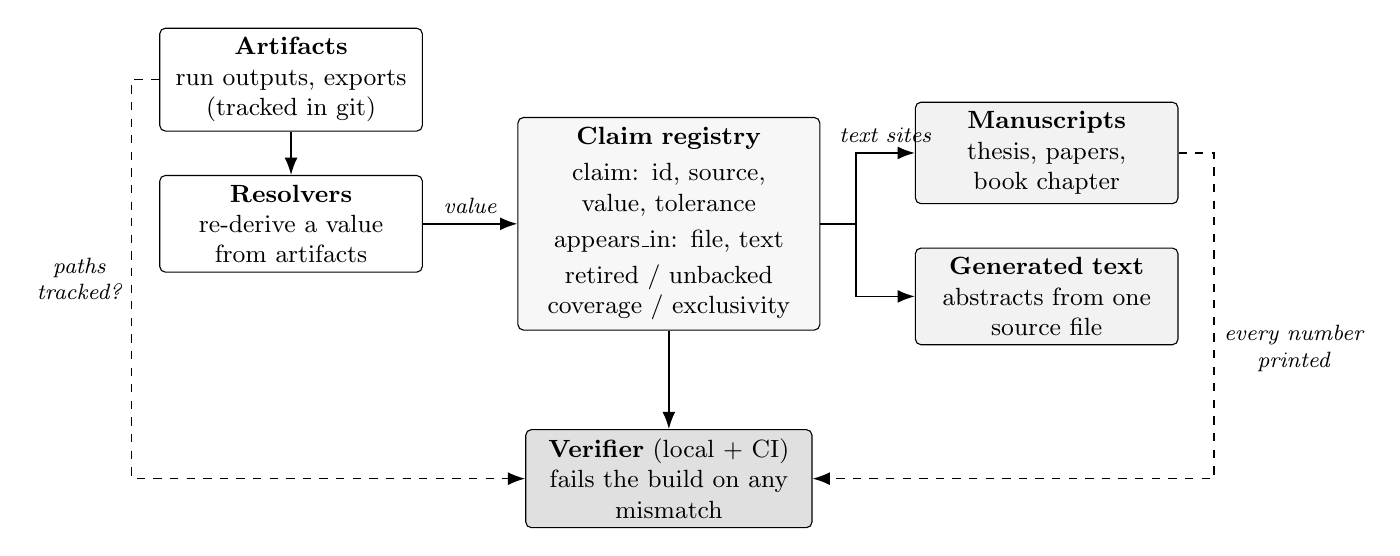
\begin{tikzpicture}[
  font=\small,
  box/.style={draw, rounded corners=2pt, align=center, minimum height=1.05cm,
              text width=3.1cm, fill=white},
  doc/.style={box, fill=black!5},
  chk/.style={box, fill=black!12, text width=3.4cm},
  arr/.style={-{Latex[length=2.2mm]}, semithick},
  lab/.style={font=\footnotesize\itshape, align=center}
]
% Left: evidence
\node[box] (art) {\textbf{Artifacts}\\ run outputs, exports\\ (tracked in git)};
\node[box, below=0.55cm of art] (res) {\textbf{Resolvers}\\ re-derive a value\\ from artifacts};
% Centre: registry
\node[box, right=1.2cm of res, text width=3.6cm, minimum height=2.7cm, fill=black!3] (reg)
  {\textbf{Claim registry}\\[2pt] claim: id, source,\\ value, tolerance\\[2pt]
   appears\_in: file, text\\[2pt] retired / unbacked\\ coverage / exclusivity};
% Right: documents
\node[doc, right=1.2cm of reg, yshift=0.9cm] (ms) {\textbf{Manuscripts}\\ thesis, papers,\\ book chapter};
\node[doc, below=0.55cm of ms] (frag) {\textbf{Generated text}\\ abstracts from one\\ source file};
% Bottom: checks
\node[chk, below=1.25cm of reg] (ver) {\textbf{Verifier} (local + CI)\\ fails the build on any\\ mismatch};
\draw[arr] (art) -- (res);
\draw[arr] (res) -- node[lab, above] {value} (reg);
\draw[arr] (reg.east) -- ++(0.45,0) |- node[lab, pos=0.75, above] {text sites} (ms.west);
\draw[arr] (reg.east) -- ++(0.45,0) |- (frag.west);
\draw[arr] (reg) -- (ver);
\draw[arr, dashed] (ms.east) -- ++(0.45,0) |- node[lab, pos=0.3, right] {every number\\ printed} (ver.east);
\draw[arr, dashed] (art.west) -- ++(-0.35,0) |- node[lab, pos=0.25, left] {paths\\ tracked?} (ver.west);
\end{tikzpicture}
\end{document}
